Machine Learning (ML) as a field has already revolutionized numerous domains, from image recognition and natural language processing to drug discovery. The success of machine learning relies on using backpropagation to optimize parameterized model functions by training them on large amounts of data.

\section{Graph Neural Networks}
Graph neural networks are a specialized variant of neural networks designed for graph-structured data. In our case, the graph represents the molecular structure of the system we want to model. Each atom acts as a node in the graph, containing information about the local density in the form of coefficients from atom-centered basis functions. The edges of the graph contain information about interatomic distances, which can be embedded as edge features in the graph neural network.
\subsection{OF-DFT Model and basis set predictor model}
For the OF-DFT we are using the architecture used in M-OFDFT\cite{zhang_m-ofdft_2023} and which is an modified Graphormer-architecture \cite{ying2021transformers}. The Graphformer is a transformer like architecture that operates on graph structured data, in this case a complete graph but takes into account the distances between different nodes in its attention module.\\
We also introduce an atomic reference module as it was done in M-OFDFT.\\
For the graph neural network that is used in chapter
\ref{chapter:adaptivebasisfunctions} to predict the exponents and coefficients of an orbital basis set we use a much smaller message passing neural network, as it is described in the following sections.

\subsection{Messagepassing Neural Network}
Message Passing Neural Networks (MPNNs) operate on graph-structured data G = (V, E), where V is the set of nodes and E is the set of edges. The core of MPNNs is the message passing operation, defined as:

\begin{align}
m_t^{(v)} &= \text{AGG}\left(\{M_t(h_t^{(v)}, h_t^{(u)}, e_{vu}) \mid u \in N(v)\}\right) \\
h_{t+1}^{(v)} &= U_t(h_t^{(v)}, m_t^{(v)})
\end{align} 
    

where $h_t^{(v)}$ is the hidden state of node $v$ at time step $t$, $e_{vu}$ is the edge feature between nodes $v$ and $u$, $N(v)$ is the neighborhood of $v$, $M_t$ is the message function, AGG is an aggregation function (e.g., sum, mean, max), and $U_t$ is the update function. These operations are performed for $T$ successive layers.

\subsubsection{Embeddings}
The embedding described here is used by the graph neural network in chapter
\ref{chapter:adaptivebasisfunctions} the embedding for the OF-DFT model is different as shifted Gaussians are used instead of besselfunctions.\\
The atomic number of every atom is one hot encoded into a vector which length the number of distinct atomtypes in the dataset is.
The distance between the atoms is embedded using besselfunction following the approach of \cite{gasteiger_directional_2022}. See figure \ref{fig:bessel_embedding}
\begin{align}
    \tilde{e}_{\text{RBF},n}(d) &= \sqrt{\frac{2}{c}}\frac{\sin(\frac{\omega_n }{c})}{d}\hspace{2cm} \omega_n :=(n+1)d\pi\\
    u(d)&= 1-\frac{(p+1)(p+2)}{2}d^p + p(p+2)d^{p+1}-\frac{p(p+1)}{2}d^{p+2}
\end{align}
Where we choose p = 1 and c = 6, as most of the bonds in our dataset are shorter than 6 Angstrom as can be seen in figure \ref{fig:bond_length}. The distance embedding is then multiplied with the one hot encoded atomic number of the atom to get the final edge feature.
\begin{figure}
    \centering
    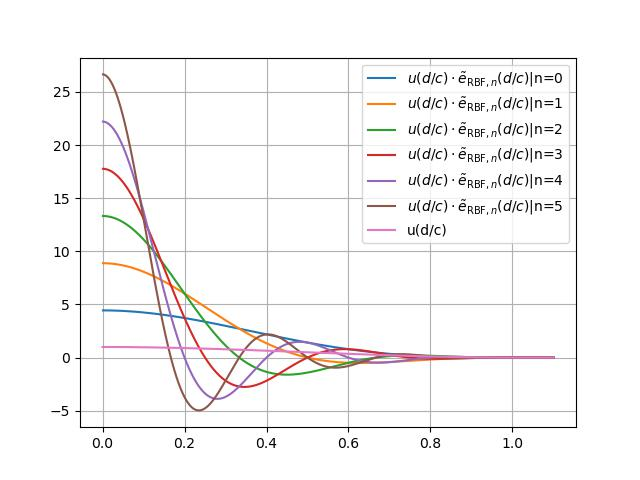
\includegraphics[width=1.\textwidth]{chapters/foundations/images_foundation/bessel_embedding}
    \caption{The initial basis function used for the distance embedding in the graph neural network from chapter
\ref{chapter:adaptivebasisfunctions}. The OF-DFT model uses shifted Gaussians instead.}
    \label{fig:bessel_embedding}
\end{figure}
\begin{figure}
    \centering
    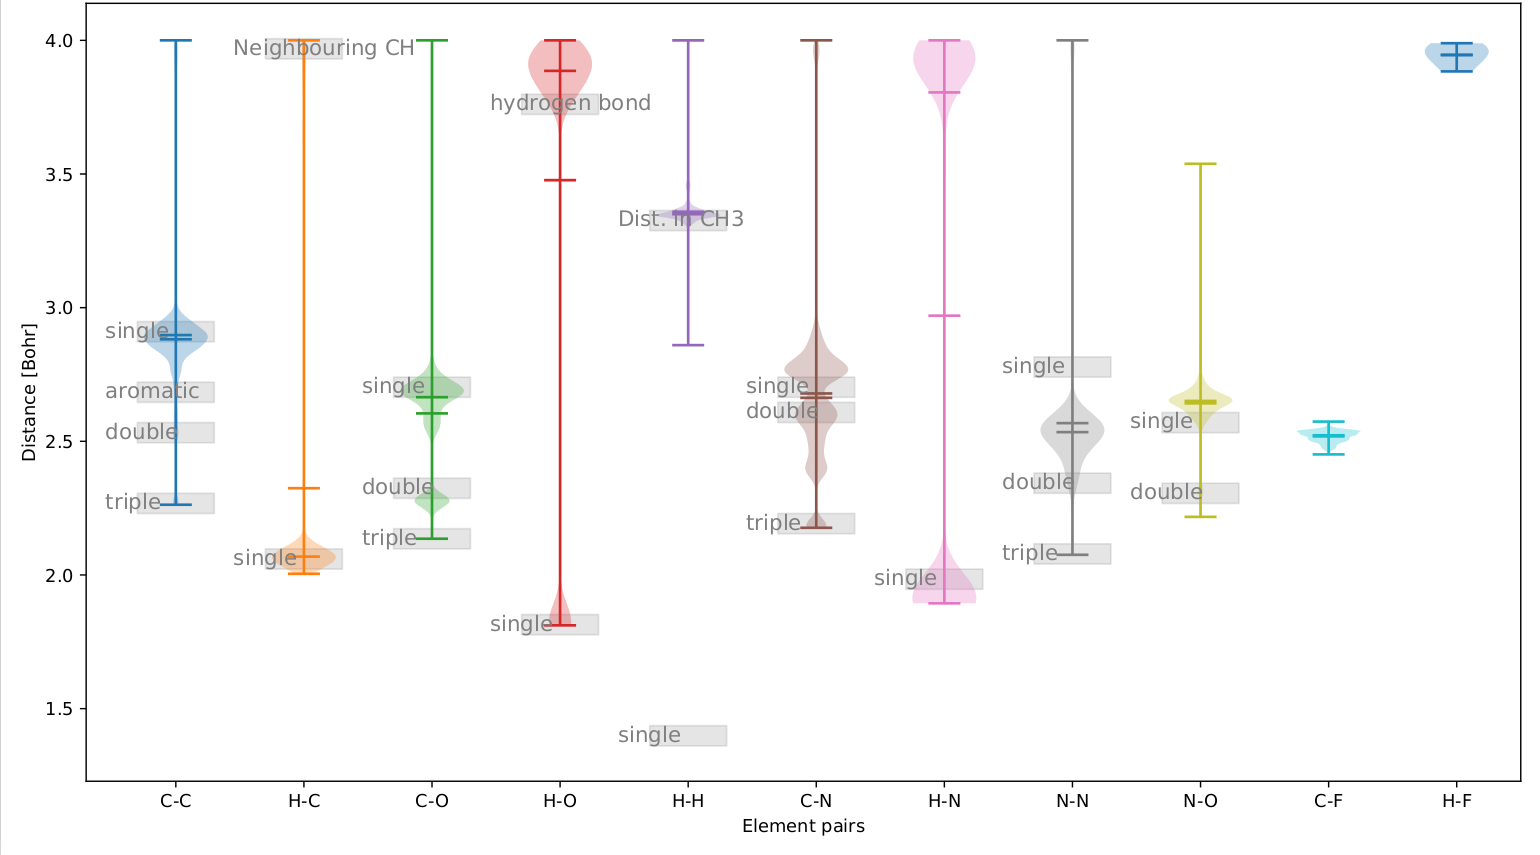
\includegraphics[width=1.\textwidth]{chapters/foundations/images_foundation/bondlength}
    \caption{The average Bondlength appearing in QM9\cite{ramakrishnan2014quantum}. The x axis show different nearest neightbor combinations while y shows the respective distances. The quantity of occurence of each dintance is visualized using a violin plot. This grafic was put together by Tobias Kaczun.}
    \label{fig:bond_length}
\end{figure}
For the final embedding of the edge features the one hot encoded atomic number of the incoming and outgoing atoms is concatenated with the distance embedding. This is then passed through a short multi layer perceptron(MLP).
%\begin{align}
%        h_i:= \text{HOTONE(z_i)}\in R^{n_z}\\
%        e_{\text{edge embedding},i,j}^{(0)} = \sigma((h_i||h_j||\text{emb_{ij}})W_{\text{edge}}+b_{\text{edge}})\\
%    e_{\text{edge embedding},i,j}^{(1)} &= u(d_{i,j})(x_{\text{edge embedding}}^{(0)} + \text{MLP}(x_{\text{edge embedding}}^{(0)}))
%\end{align}
These edge features are aggregated into node features using an aggregation function. The Node features are then futher processed.
\begin{align}
    n_{node_{features},i}^{(0)} &= \text{AGG}(e_{\text{edge embedding},i,j}^{(1)})_i + h_{i}W_{\text{node}} + b_{\text{node}} \\
    n_{node_{features},i}^{(l+1)} &= \text{BatchNorm}(n_{node_{features},i}^{(l)} + \text{MLP}(n_{node_{features},i}^{(l)}))
\end{align}
Then iteratively new edge messages are constructed from these node features and again aggregated to node features:
\begin{align}
    e_{\text{edge embedding},i,j}^{(l+1)} &= \text{MLP}(n_{node_{features}i}^{(l)}||n_{node_{features},j}^{(l)}||e_{\text{edge embedding}i,j}^{(l)})\\
    n_{node_{features},i}^{(l+1)} &= \text{AGG}(e_{\text{edge embedding},i,j}^{(l+1)})_i + n_{node_{features},i}^{(l)}
\end{align}
In the end a final MLP is used to produce a vector for each atom from which atomic properties can be predicted.

